\subsection{System and Connections}
\label{sec:system_connections}

The \texttt{System} class represents a complete co-simulation model.
It collects the participating components, stores the connections between them, and provides the structural context required for orchestration.
In this way, the definition of individual subsystem models is kept separate from the definition of the coupled system.
Figure~\ref{fig:system_architecture} illustrates this separation: the left panel shows a system as defined by the user, while the right panel shows the structural information the framework derives during initialization.

\begin{figure}[htbp]
  \centering
  \vspace{-1em}
  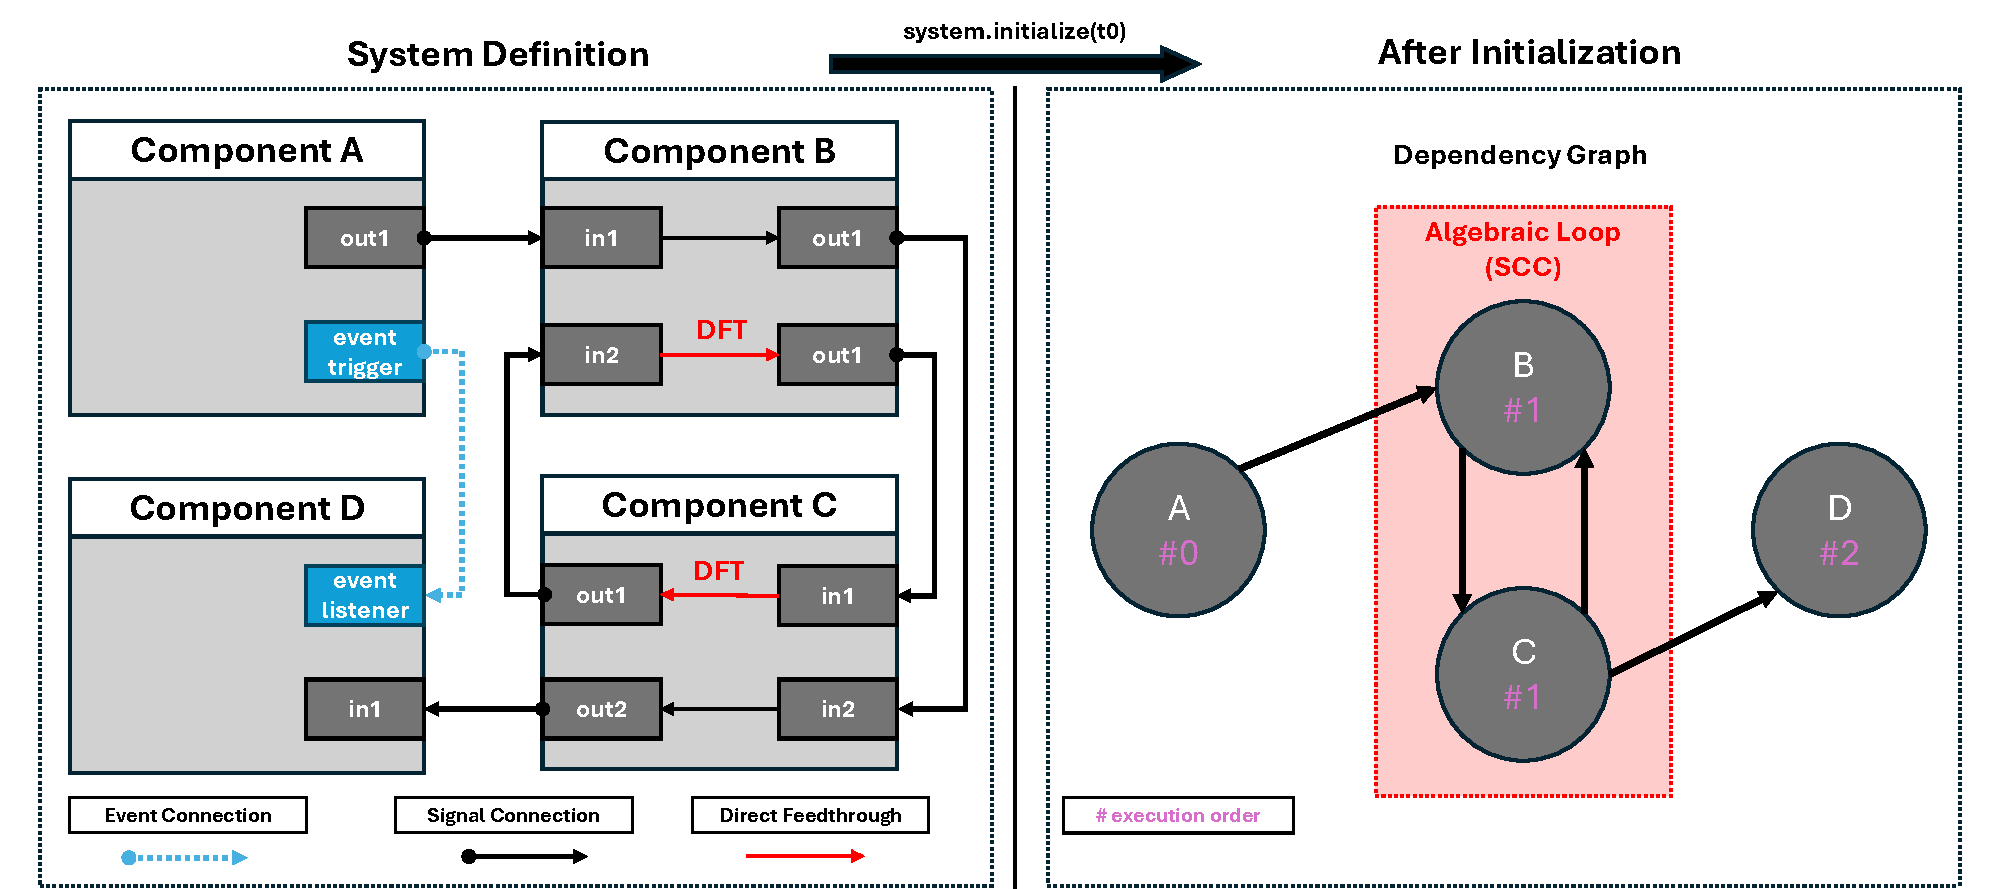
\includegraphics[width=\textwidth]{figures/4_architecture/system_architecture.pdf}
  \vspace{-1em}
  \caption{System definition and initialization. The left panel shows the user-defined system model with four components, their typed ports, signal connections (solid arrows), an event connection (dashed blue), and direct-feedthrough paths (solid red). The right panel shows the result of \texttt{system.initialize(t0)}: the framework derives a dependency graph, computes a topologically sorted execution order (\#), and identifies algebraic loops as strongly connected components (shaded region).}
  \vspace{-0.5em}    
  \label{fig:system_architecture}
\end{figure}

Two types of connections are supported.
A signal connection defines a directed data flow from an output port of a source component to an input port of a destination component.
An event connection routes a named event from a source component to a handler method in a destination component, enabling cross-component discrete interactions such as mode changes or contact triggers.
Both connection types are visible in Figure~\ref{fig:system_architecture} (left): solid arrows denote signal connections, while the dashed arrow represents an event connection.
When a connection is added, the \texttt{System} validates that the referenced ports exist and that the connected ports are type- and unit-compatible.

From the registered components and connections, the \texttt{System} builds a dependency graph in which components form the nodes and directed connections form the edges.
This graph is the basis for the structural analysis performed during initialization: the framework derives a topologically sorted execution order, identifies direct-feedthrough dependencies, and detects algebraic loops.
As shown in Figure~\ref{fig:system_architecture} (right), components~B and~C form a strongly connected component due to their mutual direct-feedthrough dependencies, which the framework flags as an algebraic loop.
The details of these analyses are discussed in Chapter~\ref{chap:implementation}; at the architectural level, it is sufficient to note that they are computed automatically and made available to the execution algorithms.

The \texttt{System} class does not implement a stepping scheme itself.
Instead, it holds a reference to an \texttt{Algorithm} object and delegates the simulation loop to it.
